\documentclass[conference]{IEEEtran}

\usepackage[T1]{fontenc}
\usepackage[utf8]{inputenc}
\usepackage[brazil]{babel}
\usepackage{amsmath}
\usepackage{array}
\usepackage{cite}
\usepackage{graphicx}
\usepackage{tabularx}
\usepackage{url}

\newcolumntype{Y}{>{\raggedright\arraybackslash}X}
\newcommand{\NA}{não caracterizado}

\title{BioDiff-CMOS: projeto pré-silício e verificação física de um bloco diferencial CMOS para aquisição simulada de ECG}

\author{
\IEEEauthorblockN{Danilo da Silva Cunha, André Felipe Feitosa de Souza, Fábio de Sousa Cardoso, Isabela Rogério Cardoso,\\
André Luiz Printes, Afonso Aguiar de Carvalho, Jozias Parente de Oliveira e Angilberto Muniz Ferreira Sobrinho}
\IEEEauthorblockA{CI Amazônia e Universidade do Estado do Amazonas, Manaus, AM, Brasil\\
Autor para correspondência: dsc.elt@uea.edu.br}
}

\begin{document}
\maketitle

\begin{abstract}
Este artigo apresenta o projeto pré-silício e a verificação física do BioDiff-CMOS, um bloco diferencial para uma cadeia simulada de aquisição de eletrocardiograma (ECG), no processo IHP SG13G2 BiCMOS de 130~nm. O fluxo reproduzível utiliza Xschem, Ngspice, Magic e Netgen e inclui simulação em nível esquemático, layout, extração, simulação pós-layout, verificação de regras de projeto e comparação entre layout e esquemático. Na condição nominal típica, a 1,8~V e 27~$^{\circ}$C, o núcleo apresentou ganho diferencial de 0,908~V/V em 100~Hz, ruído referido à entrada de 29,93~$\mu$V$_{\mathrm{rms}}$ entre 0,5 e 150~Hz, CMRR nominal de 128,3~dB em 100~Hz e consumo de 36,01~$\mu$W. O filtro RC de primeira ordem apresentou corte de $-3$~dB em 120,884~Hz. O DRC não reportou violações no conjunto de regras executado e o LVS apresentou correspondência única de conectividade. A extração usada nesta versão contém 18 capacitâncias e não contém resistências parasitas de interconexão, portanto os resultados pós-layout são classificados como capacitivos e híbridos. O circuito não foi fabricado e não houve aquisição de ECG real. Os resultados documentam um estudo de caso pré-silício, sem validar um sistema biomédico nem demonstrar robustez a descasamento.
\end{abstract}

\begin{IEEEkeywords}
ECG, amplificador diferencial CMOS, front-end analógico, projeto pré-silício, verificação física.
\end{IEEEkeywords}

\section{Introdução}

O eletrocardiograma (ECG) é um biopotencial de baixa amplitude e baixa frequência. Sua aquisição requer alta impedância de entrada, rejeição de interferência em modo comum, baixo ruído e consumo compatível com aplicações portáteis. Circuitos integrados recentes combinam amplificação, filtragem e técnicas de estabilização para atender a esses requisitos \cite{wen2025,kim2016,zhao2019}. O ganho, a razão de rejeição de modo comum (CMRR), o ruído referido à entrada e a potência devem ser avaliados junto com a banda, a carga, o processo e o estado de validação do circuito.

Kits de projeto de processo (PDKs) abertos e ferramentas de automação de projeto eletrônico (EDA) permitem estudar o percurso entre a descrição elétrica e o layout. Nesse fluxo, a verificação de regras de projeto (DRC) avalia a geometria e a comparação layout versus esquemático (LVS) verifica a conectividade. Nenhuma dessas etapas mede desempenho em silício ou substitui a caracterização experimental.

Este trabalho implementa e verifica por simulação, DRC e LVS o BioDiff-CMOS no processo IHP SG13G2. A contribuição é um estudo de caso rastreável, com os mesmos estímulos nas análises pré e pós-layout, caracterização nominal adicional, triagem de cinco pontos de processo, tensão e temperatura (PVT) e documentação explícita dos limites da extração. O trabalho não apresenta chip fabricado, medições de bancada ou aquisição de ECG.

\section{Trabalhos relacionados}

A Tabela~\ref{tab:literatura} compara o BioDiff-CMOS com front-ends representativos. Kim e Ko \cite{kim2016} e Zhao, Shang e Lian \cite{zhao2019} reportaram silício medido. Laababid, El Khadiri e Tahiri \cite{laababid2022} e Wen \emph{et al.} \cite{wen2025} reportaram simulações em 180~nm. As unidades foram uniformizadas, mas os escopos permanecem diferentes: alguns valores representam um amplificador de instrumentação, outros um canal completo, e a área pode se referir ao núcleo ou ao chip.

\begin{table*}[t]
\caption{Comparação com front-ends analógicos representativos da literatura.}
\label{tab:literatura}
\centering
\scriptsize
\setlength{\tabcolsep}{3pt}
\begin{tabularx}{\textwidth}{p{2.25cm} p{2.65cm} p{1.7cm} p{1.45cm} p{2.35cm} p{1.55cm} Y}
\hline
Trabalho & Estado, processo e $V_{DD}$ & Ganho & CMRR & Ruído referido à entrada & Potência & Banda, área e observações \\
\hline
BioDiff-CMOS & Pré/pós-layout híbrido; IHP 130~nm; 1,8~V & $-0,835$~dB em 100~Hz & 128,3~dB em 100~Hz, nominal & 29,93~$\mu$V$_{\mathrm{rms}}$, 0,5--150~Hz & 36,01~$\mu$W, cadeia simulada & Corte de 120,884~Hz; núcleo: 0,00093456~mm$^2$; fonte de cauda ideal \\
Kim e Ko \cite{kim2016} & Fabricado e medido; CMOS 130~nm; 1,2~V & 44,7~dB em 60~Hz & 91,3~dB em 60~Hz & 0,92~$\mu$V$_{\mathrm{rms}}$, banda de 100~Hz & 6~$\mu$W, IA em PG+CS & Filtro de 100~Hz; área da IA não reportada; die de 6,02~mm$^2$ \\
Zhao \emph{et al.} \cite{zhao2019} & Fabricado e medido; CMOS 350~nm; 1,8~V & 56--68~dB & 76~dB & 1,02~$\mu$V$_{\mathrm{rms}}$, 0,4--120~Hz & 0,90~$\mu$W & 0,4--120~Hz; 0,405~mm$^2$ \\
Laababid \emph{et al.} \cite{laababid2022} & Simulação esquemática; CMOS 180~nm; 1,8~V & 50,75~dB em 20~Hz & 102~dB & 1,47~$\mu$V$_{\mathrm{rms}}$, 0,1~Hz--1~kHz & 1,08~$\mu$W & 0,077--255~Hz no corpo do artigo; área não reportada \\
Wen \emph{et al.} \cite{wen2025} & Simulação TT; CMOS 180~nm; 1,8~V & 29,5--47,6~dB & $>114$~dB & 8,538~$\mu$V$_{\mathrm{rms}}$, 0,5--150~Hz & 84,4~$\mu$W, inferidos & Canal de amostragem; saída e RLD excluídos; área não reportada \\
\hline
\end{tabularx}
\end{table*}

O núcleo deste trabalho tem ganho inferior à unidade e fica de 30 a 69~dB abaixo dos ganhos listados. O ruído integrado é cerca de 3,5 vezes o valor de Wen \emph{et al.} e mais de 29 vezes os valores medidos por Kim e Ko e por Zhao \emph{et al.} O CMRR nominal parece superior, mas foi obtido com fonte de cauda ideal, simetria determinística e sem descasamento, condição que favorece artificialmente essa métrica. A potência de 36,01~$\mu$W fica entre os valores comparados, porém inclui a interface CMOS simulada e exclui um circuito físico de polarização. Portanto, a comparação identifica lacunas de desempenho e não estabelece uma classificação direta.

\section{Materiais e métodos}

\subsection{Circuito e condições de teste}

O núcleo possui dois NMOS de entrada com razão largura/comprimento $W/L=3,2/0,8~\mu$m e duas cargas \texttt{rhigh} de $2/10~\mu$m. Uma fonte ideal fornece 20~$\mu$A ao nó de cauda. A saída positiva alimenta um ramo de 1,33~M$\Omega$/1~nF e as portas de um inversor e de um buffer CMOS. A saída negativa não recebe carga externa equivalente. A Fig.~\ref{fig:schematic} distingue o núcleo implementado no layout da carga e da interface do testbench. A interface não implementa amostragem, quantização nem taxa de conversão, por isso não é tratada como conversor analógico-digital.

\begin{figure*}[t]
\centering
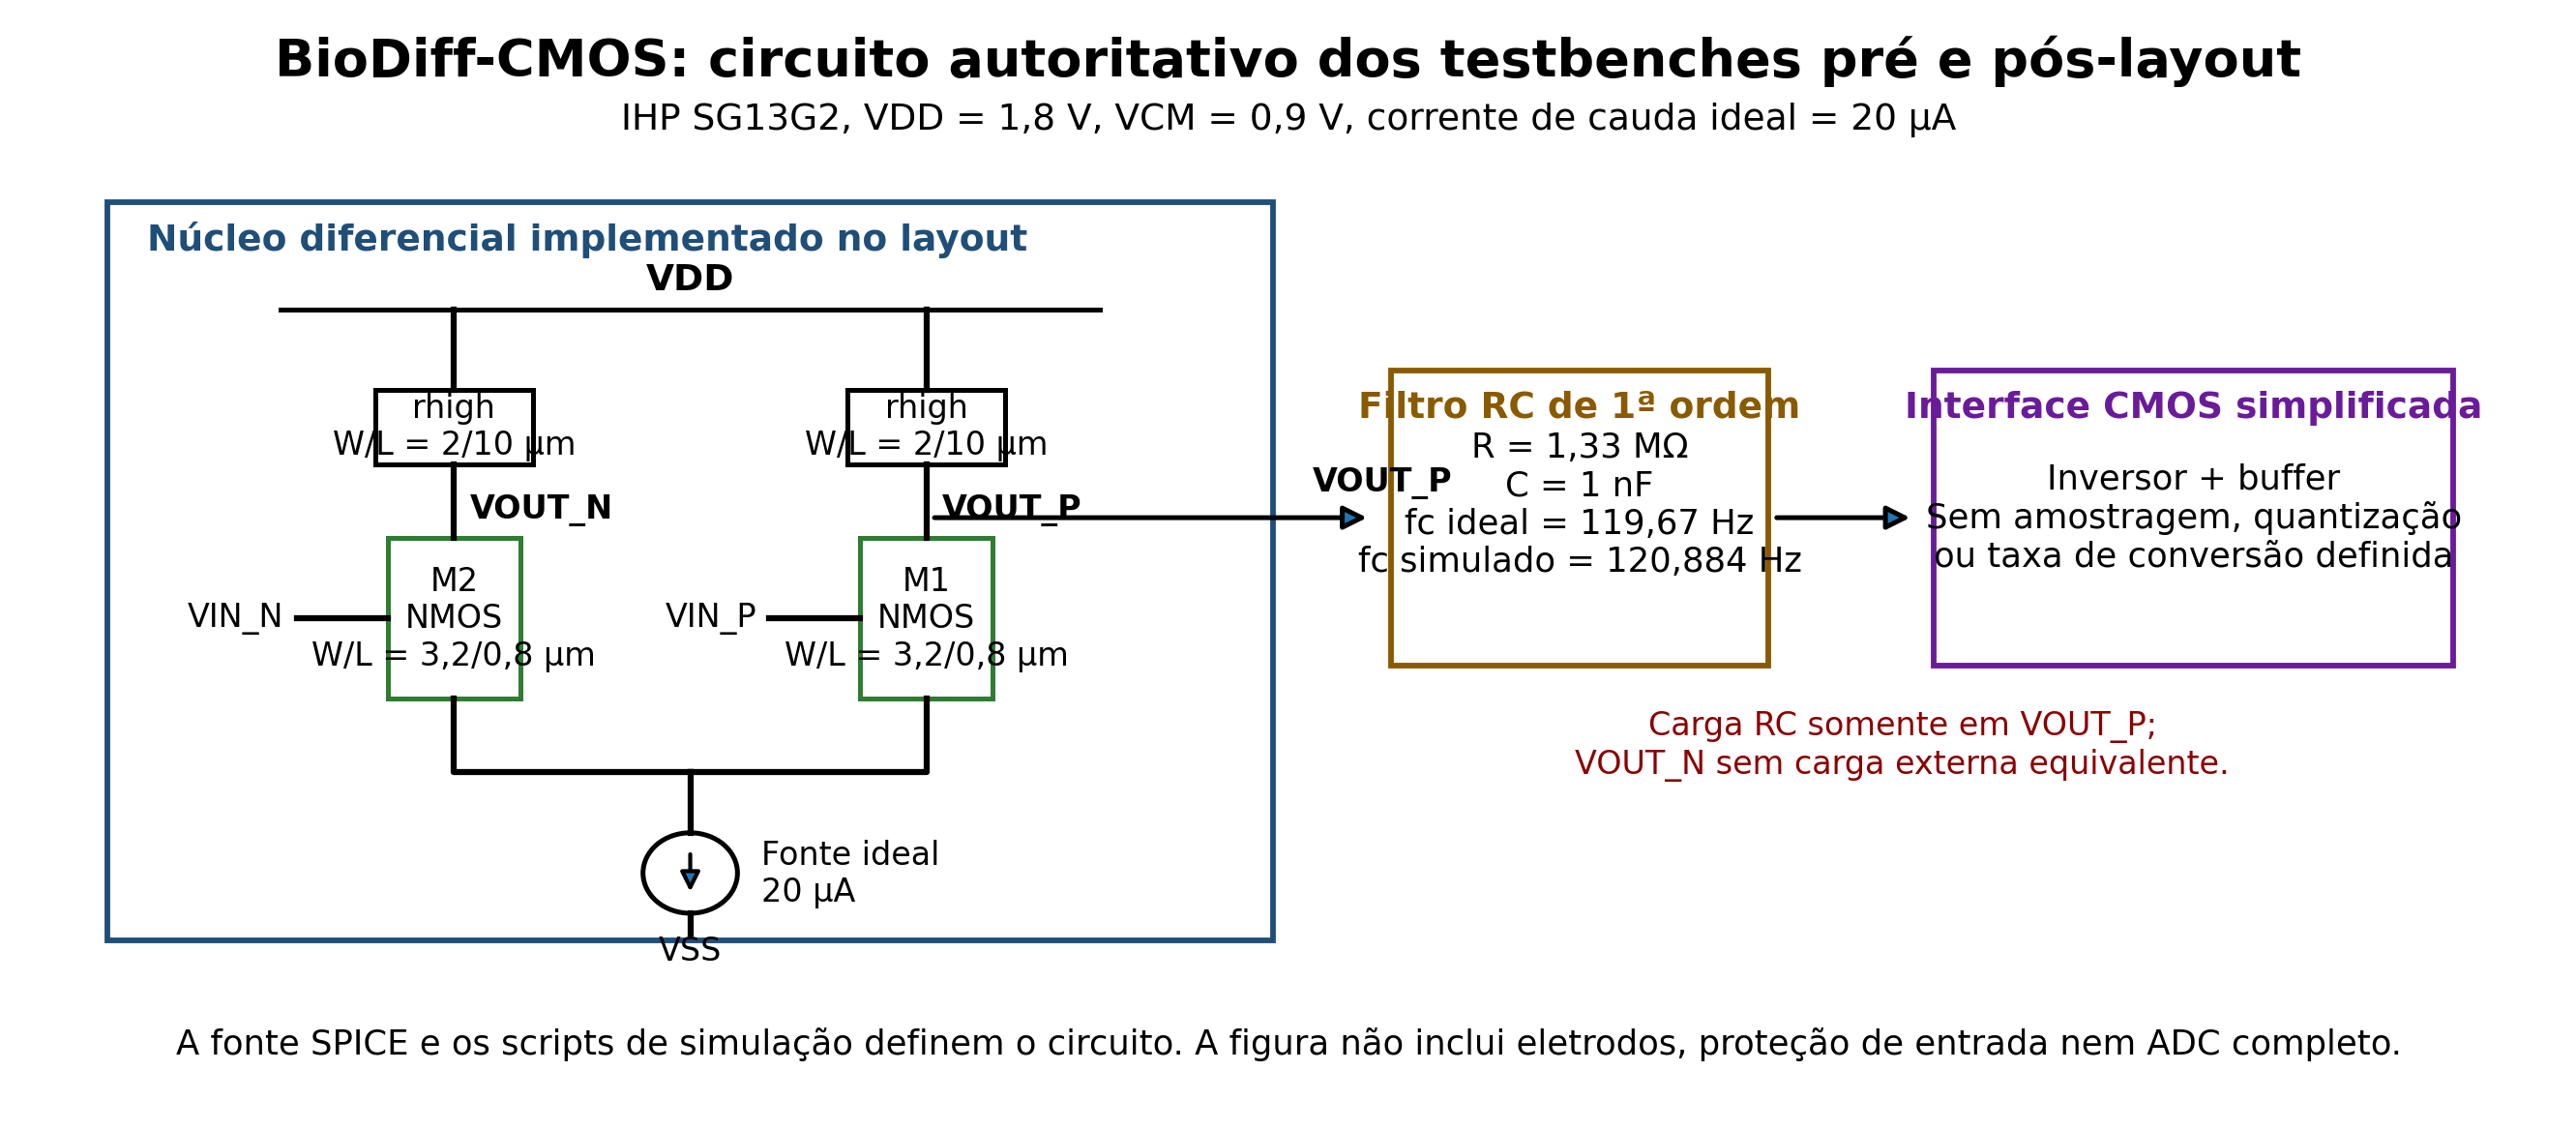
\includegraphics[width=0.96\textwidth]{figures/schematic.png}
\caption{Circuito definido pelas netlists dos testbenches. Somente o núcleo dentro do quadro azul foi implementado no layout.}
\label{fig:schematic}
\end{figure*}

As análises pré e pós-layout utilizaram o mesmo testbench; somente a netlist do núcleo foi substituída. A condição nominal usou os modelos \texttt{mos\_tt}, \texttt{res\_typ} e \texttt{cap\_typ}, 27~$^{\circ}$C, 1,8~V e modo comum de entrada de 0,9~V. A análise AC aplicou 1~V diferencial, dividido em $+0,5$ e $-0,5$~V. O ensaio transiente aplicou 25~mV de pico por entrada em oposição de fase, equivalentes a 100~mV$_{pp}$ diferenciais em 1~kHz. Esse ensaio é elétrico e não representa um ECG.

O ruído referido à entrada foi integrado entre 0,5 e 150~Hz e, como verificação complementar, entre 0,05 e 150~Hz. CMRR e razão de rejeição da alimentação positiva (PSRR+) foram calculados na saída diferencial. O offset nominal foi obtido por varredura DC, sem modelos estatísticos. O circuito ideal de cauda permite tensões não físicas em modo comum baixo, portanto a faixa de modo comum de entrada (ICMR) não foi reportada.

\subsection{Layout, extração e reprodutibilidade}

O layout da Fig.~\ref{fig:layout} foi criado no Magic com simetria entre os dispositivos de entrada. O bounding box da geometria pintada, sem marcadores, pads ou área de die, mede 26,40 por 35,40~$\mu$m, ou 934,56~$\mu$m$^2$. O DRC foi executado com o deck do IHP SG13G2. O LVS comparou sete pinos e quatro instâncias; as classes \texttt{sg13\_lv\_nmos} e \texttt{rhigh} foram tratadas como caixas-pretas equivalentes.

\begin{figure}[t]
\centering
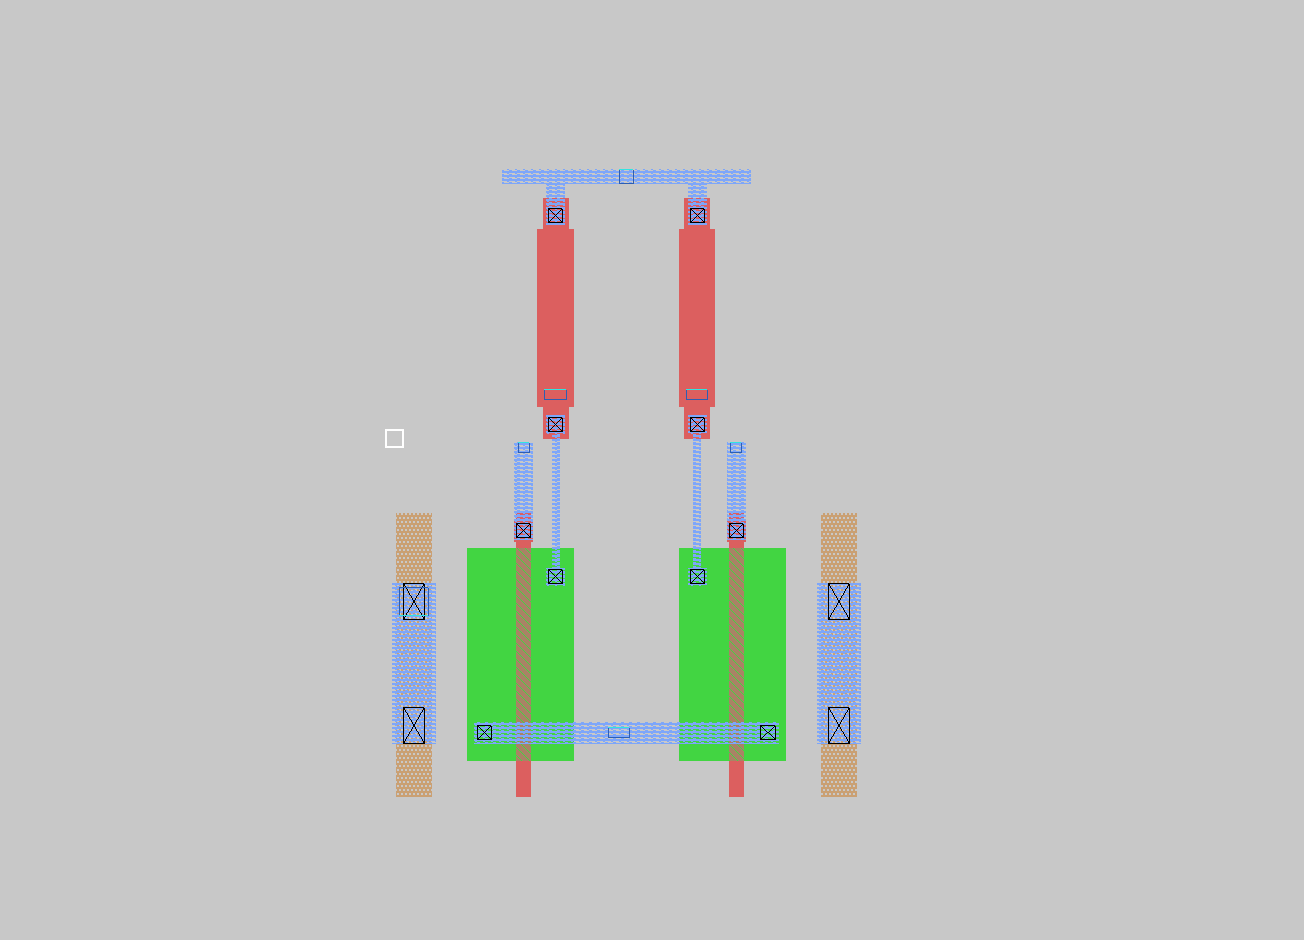
\includegraphics[width=\columnwidth]{figures/layout_full.png}
\caption{Layout do núcleo diferencial no processo IHP SG13G2.}
\label{fig:layout}
\end{figure}

A extração no Magic usou \texttt{extract do local}, \texttt{extract all}, \texttt{ext2spice lvs}, limiar capacitivo zero e extração resistiva habilitada. A netlist resultante desta versão contém 18 capacitâncias, nenhum resistor parasita de interconexão e duas cargas \texttt{rhigh} reconstruídas para compatibilidade do testbench. Assim, a análise é pós-layout capacitiva e híbrida, não uma PEX RC completa.

O ambiente reproduzível usa a imagem \texttt{isaiassh/unic-cass-tools:1.1.0}, PDK IHP Open PDK v0.3.0 no commit \texttt{5cccb161f749}, Ngspice 44.2, Magic 8.3.613, Netgen 1.5.293 e Xschem no commit \texttt{313acc8e2974}. Os arquivos mínimos são as netlists em \texttt{entrega/sim\_pre} e \texttt{entrega/pex\_post}, a célula \texttt{entrega/layout/biodiff\_top.mag} e os scripts em \texttt{scripts/entrega}. Os comandos e os artefatos gerados são descritos no repositório do projeto \cite{repo}.

\section{Resultados}

\subsection{Caracterização nominal pré e pós-layout}

A Tabela~\ref{tab:specs} consolida as condições e as métricas solicitadas. Os resultados pré e pós-layout coincidem na precisão apresentada para ganho, ruído, corte e potência. Essa coincidência decorre da pequena carga capacitiva extraída e não demonstra robustez de fabricação.

\begin{table*}[t]
\caption{Especificações e resultados consolidados do BioDiff-CMOS.}
\label{tab:specs}
\centering
\scriptsize
\setlength{\tabcolsep}{4pt}
\begin{tabularx}{\textwidth}{p{3.1cm} Y p{2.25cm} p{2.25cm} p{2.6cm}}
\hline
Parâmetro & Condição ou definição & Pré-layout & Pós-layout & Unidade ou observação \\
\hline
PDK e processo & IHP SG13G2 BiCMOS & 130 & 130 & nm \\
Alimentação & Fonte principal & 1,8 & 1,8 & V \\
Dispositivos do núcleo & NMOS de entrada; cargas \texttt{rhigh} & 3,2/0,8; 2/10 & 3,2/0,8; 2/10 & $W/L$ em $\mu$m \\
Interface CMOS & Inversor PMOS/NMOS; buffer PMOS/NMOS & 4/0,35; 2/0,35; 8/0,35; 4/0,35 & mesma & $W/L$ em $\mu$m; fora do layout do núcleo \\
Corrente de polarização & Fonte de cauda ideal & 20 & 20 & $\mu$A; circuito de polarização não implementado \\
Modo comum nominal & Entradas & 0,9 & 0,9 & V \\
Ganho diferencial & 10; 100; 1000~Hz & 0,909260; 0,908323; 0,906963 & 0,909260; 0,908323; 0,906963 & V/V \\
Corte do filtro & $-3$~dB relativo a 1~Hz & 120,884 & 120,884 & Hz \\
ICMR & Fonte de cauda ideal invalida o limite inferior & \NA & \NA & Requer polarização física \\
Excursão de saída & Extremos da varredura DC diferencial & 0,286523 & 0,286523 & V$_{pp}$ diferencial; faixa linear não qualificada \\
CMRR & Saída diferencial, 100~Hz & 128,292 & 128,291 & dB; otimista, sem descasamento \\
PSRR+ & Saída diferencial, 100~Hz & 48,683 & 48,683 & dB; polarização ideal \\
Ruído referido à entrada & Integrado, 0,5--150~Hz & 29,9317 & 29,9317 & $\mu$V$_{\mathrm{rms}}$ \\
Ruído referido à entrada & Integrado, 0,05--150~Hz & 35,4578 & 35,4578 & $\mu$V$_{\mathrm{rms}}$ \\
Offset nominal & Varredura DC, sem descasamento & $-25,32$ & $-25,32$ & $\mu$V; não representa offset de fabricação \\
Potência & Média na fonte de 1,8~V & 36,0116 & 36,0116 & $\mu$W; polarização física excluída \\
Área do núcleo & Bounding box da geometria & 934,56 & 934,56 & $\mu$m$^2$; sem pads \\
Carga & Somente em \texttt{VOUT\_P} & 1,33~M$\Omega$/1~nF + portas CMOS & mesma & \texttt{VOUT\_N} sem carga externa equivalente \\
Corner e temperatura & Modelos MOS/R/C & TT/típico/típico; 27 & TT/típico/típico; 27 & $^{\circ}$C \\
Extração & Elementos dentro do núcleo & nenhuma & 18 C; 0 R parasitas; 2 \texttt{rhigh} reconstruídas & Modelo pós-layout híbrido \\
DRC/LVS & Deck executado e conectividade & não aplicável & 0 violações; correspondência única & Não constitui validação elétrica \\
\hline
\end{tabularx}
\end{table*}

A resposta em frequência é mostrada na Fig.~\ref{fig:ac}. O valor de 120,884~Hz foi medido em relação ao ganho de baixa frequência. Ele está próximo dos 119,67~Hz calculados por $f_c=(2\pi RC)^{-1}$ para 1,33~M$\Omega$ e 1~nF. Usar 100~Hz como referência de $-3$~dB deslocaria indevidamente o cruzamento, pois esse ponto já se encontra atenuado.

\begin{figure}[t]
\centering
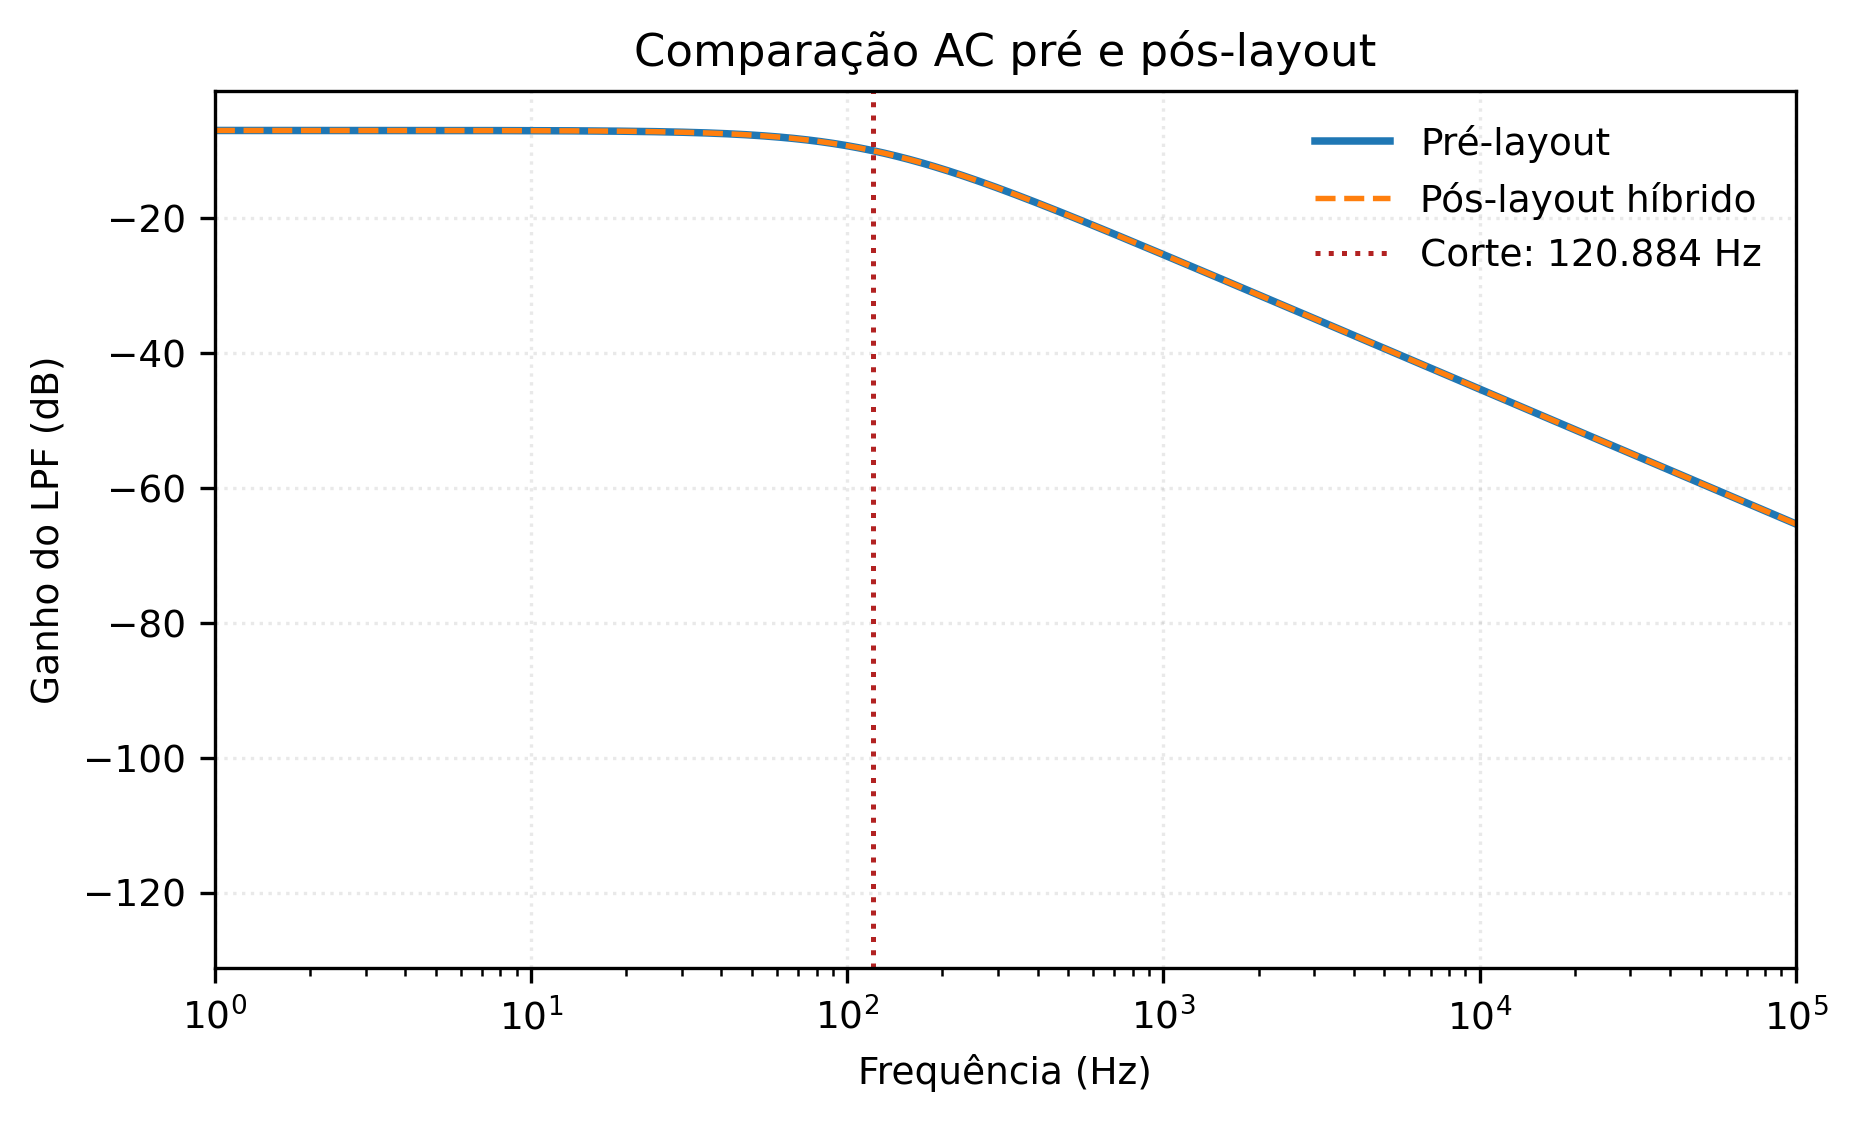
\includegraphics[width=\columnwidth]{figures/post_ac_gain.png}
\caption{Resposta AC pré e pós-layout. As curvas se sobrepõem na escala apresentada.}
\label{fig:ac}
\end{figure}

Wen \emph{et al.} adotam 0,5--150~Hz para ECG \cite{wen2025}. O corte de 120,884~Hz atenua o limite superior dessa faixa e pode ser aceitável apenas quando a aplicação permitir menor banda. Além disso, um filtro de primeira ordem tem rejeição limitada e o projeto não define taxa de amostragem, resolução ou resposta do conversor. Portanto, o ramo RC não forma sozinho uma cadeia anti-aliasing validada.

\subsection{Triagem PVT e verificações físicas}

A triagem de cinco pontos combinou TT nominal, SS em baixa tensão e alta temperatura, FF em alta tensão e baixa temperatura, e os cantos cruzados SF e FS. Como mostra a Fig.~\ref{fig:pvt}, o ganho em 1~kHz variou de 0,823 a 1,005~V/V, o corte de 119,422 a 124,297~Hz e a potência de 32,409 a 39,631~$\mu$W. Os pontos pré e pós-layout permaneceram sobrepostos. Essa triagem não substitui todos os cantos qualificados pelo PDK nem a análise de Monte Carlo.

\begin{figure}[!t]
\centering
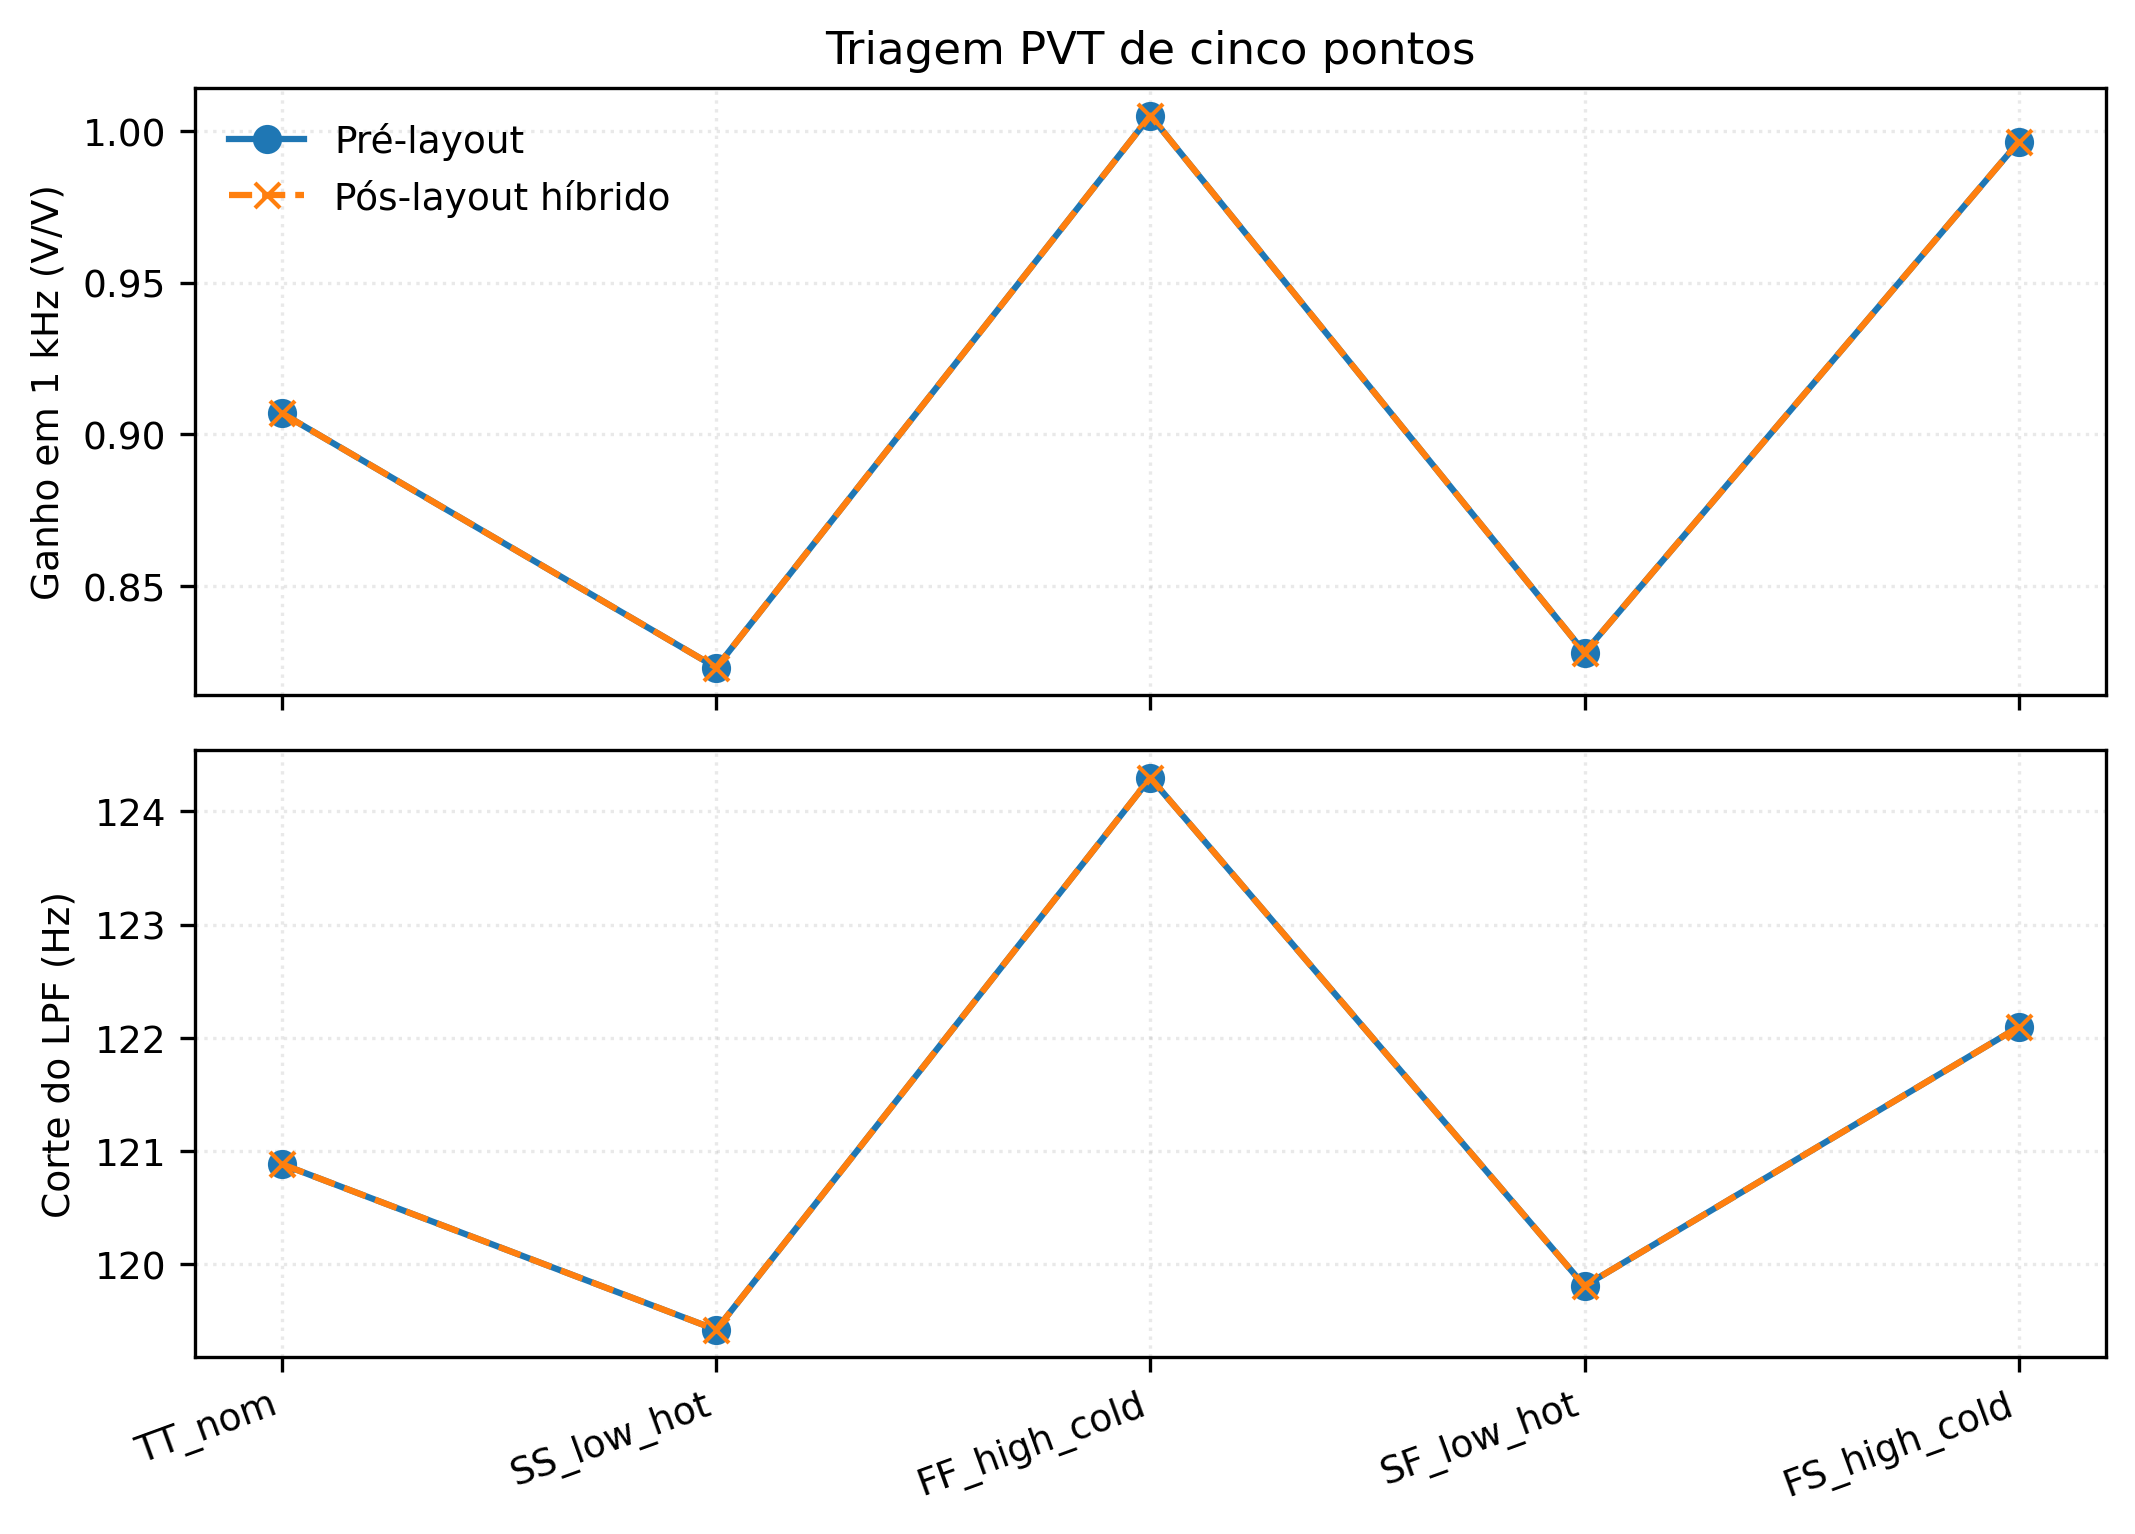
\includegraphics[width=\columnwidth]{figures/pvt_screening.png}
\caption{Triagem PVT de cinco pontos para ganho e corte do filtro.}
\label{fig:pvt}
\end{figure}

O DRC reportou zero violações no conjunto de regras executado. O LVS encontrou correspondência única entre os sete pinos e as quatro instâncias do núcleo. Esses resultados confirmam conformidade geométrica no deck usado e consistência topológica. Eles não verificam desempenho, confiabilidade, encapsulamento, fabricabilidade além do deck ou comportamento em silício.

\section{Limitações e validação futura}

As limitações dominantes são o ganho inferior à unidade, o ruído elevado em relação aos trabalhos comparados, a fonte de cauda ideal, a carga assimétrica, a PEX sem resistências de interconexão e a ausência de descasamento estatístico. O CMRR nominal não deve ser interpretado como previsão de medição. Também não foram modelados eletrodos, impedância pele-eletrodo, offset de eletrodo, interferência de 50/60~Hz ou proteção de entrada.

A validação futura seguirá três etapas. Primeiro, o projeto pré-silício será ampliado com todos os cantos definidos pelo PDK, Monte Carlo, modelos de eletrodos, offset, interferência de rede e sinais públicos de ECG. Depois, serão integrados polarização física, proteção de entrada, ganho adicional e interface de saída, seguidos por nova PEX RC, DRC e LVS. Uma fabricação em rodada multiprojeto (MPW) dependerá do atendimento às especificações e da disponibilidade de uma rodada compatível. Se houver fabricação, uma placa de teste caracterizará ganho, banda, CMRR, PSRR, ruído, offset, ICMR, excursão e potência sob carga conhecida. Os ensaios iniciais usarão um simulador de ECG; aquisição em seres humanos exigirá protocolo ético e instrumentação de segurança.

\section{Conclusão}

O BioDiff-CMOS concluiu um fluxo pré-silício reproduzível no IHP SG13G2, com simulação pré-layout, layout, extração capacitiva/híbrida, simulação pós-layout, DRC e LVS. Na condição nominal, o núcleo apresentou 0,908~V/V em 100~Hz, corte de 120,884~Hz, ruído de 29,93~$\mu$V$_{\mathrm{rms}}$ entre 0,5 e 150~Hz e 36,01~$\mu$W. O DRC não reportou violações no deck executado e o LVS confirmou conectividade única, sem validar desempenho experimental. A comparação com a literatura mostra que ganho, ruído, polarização e robustez a descasamento precisam ser revistos antes de considerar fabricação. O resultado é um estudo de caso de projeto e verificação, não um sistema biomédico validado.

\section*{Agradecimentos}

Os autores agradecem ao CI Amazônia, à Universidade do Estado do Amazonas e ao programa de capacitação em microeletrônica pelo apoio acadêmico e tecnológico.

\begin{thebibliography}{00}

\bibitem{wen2025}
Y. Wen, W. Liu, W. Li, B. Zheng, L. Dong e Q. Feng, ``An analog front-end with high common-mode rejection ratio and high input impedance for single-lead ECG signal acquisition,'' \emph{IEICE Electronics Express}, vol. 22, no. 10, Art. 20250097, 2025, doi: 10.1587/elex.22.20250097.

\bibitem{kim2016}
J. Kim e H. Ko, ``A dynamic instrumentation amplifier for low-power and low-noise biopotential acquisition,'' \emph{Sensors}, vol. 16, no. 3, Art. 354, 2016, doi: 10.3390/s16030354.

\bibitem{zhao2019}
Y. Zhao, Z. Shang e Y. Lian, ``A 2.55 NEF 76 dB CMRR DC-coupled fully differential difference amplifier based analog front end for wearable biomedical sensors,'' \emph{IEEE Trans. Biomed. Circuits Syst.}, vol. 13, no. 5, pp. 918--926, 2019, doi: 10.1109/TBCAS.2019.2924416.

\bibitem{laababid2022}
Y. Laababid, K. El Khadiri e A. Tahiri, ``Design of a low-power low-noise ECG amplifier for smart wearable devices using 180nm CMOS technology,'' \emph{WSEAS Trans. Power Syst.}, vol. 17, pp. 177--186, 2022, doi: 10.37394/232016.2022.17.18.

\bibitem{ihppdk}
IHP Microelectronics, ``IHP-Open-PDK: 130 nm BiCMOS open source PDK,'' v0.3.0, 2026. [Online]. Disponível em: \url{https://github.com/IHP-GmbH/IHP-Open-PDK}.

\bibitem{xschem}
S. Schippers, ``Xschem schematic editor,'' 2025. [Online]. Disponível em: \url{https://xschem.sourceforge.io/stefan/index.html}.

\bibitem{ngspice}
Ngspice Project, ``Ngspice open source circuit simulator,'' versão 44.2, 2025. [Online]. Disponível em: \url{https://ngspice.sourceforge.io/}.

\bibitem{magic}
Open Circuit Design, ``Magic VLSI layout tool,'' versão 8.3.613, 2026. [Online]. Disponível em: \url{http://opencircuitdesign.com/magic/}.

\bibitem{netgen}
Open Circuit Design, ``Netgen circuit netlist comparison,'' versão 1.5.293, 2026. [Online]. Disponível em: \url{http://opencircuitdesign.com/netgen/}.

\bibitem{repo}
D. S. Cunha, ``BioDiff-CMOS: arquivos de projeto e reprodução,'' 2026. [Online]. Disponível em: \url{https://github.com/DaniloCunh-a/ueletronica_projeto_final}.

\end{thebibliography}

\end{document}
